\chapter{Discussion}

This section discusses the results obtained from using sample-based metrics with possible interpretations. The best-performing model from the fine-tuning-based approach and feature-based approach is further evaluated on manually selected samples. Section \ref{quantitative_analysis} discusses a quantitative comparative analysis of language models and baselines with sample-based metrics. Section \ref{Qualitative_analysis} analyzes the quality of the best performing model from the fine-tuning-based approach and feature-based approach by evaluating some manually generated sentences.


\section{Quantitative analysis} \label{quantitative_analysis}
This section deals with quantitative analysis of language models and baselines using sample based metrics. Label based metrics and other significant properties are also discussed and compared in this analysis. 


Since it's important in our multi-label setup to identify whether a sample is a stereotype or anti-stereotype/unrelated, these categories must be ranked higher than others. Considering a case of partial matches with bias types categories (gender, ethnicity etc.) and excluding stereotype and anti-stereotype/unrelated categories might be a bit misleading. In this case, subset accuracy is simple, harsh, but a good measure as the exact match for the ground truth label is considered, thus giving equal importance to every label, including stereotype and anti-stereotype. Hence, subset accuracy is considered an important metric among the sample based metrics when doing quantitative analysis.
% Sample-based metrics were used to evaluate the performance of language models and baselines. Since it's important in our multi-label setup to identify whether a sample is a stereotype or anti-stereotype/unrelated, these categories must be ranked higher than others. Considering partial matches with bias types categories (gender, ethnicity etc.) and excluding stereotype and anti-stereotype/unrelated categories might be a bit misleading. In this case, subset accuracy is simple, harsh, but a good measure as the exact match for the ground truth label is considered, thus giving equal importance to every label, including stereotype and anti-stereotype. Hence, subset accuracy is considered an important metric among the sample based metrics when doing quantitative analysis. Other metrics such as label based metrics and  precision recall and f1-scores per class label are also being considered as parameters for quantitative analysis.

% \textbf{Test for synonyms...} on machine learning and language model to be done

\subsection{Evaluation of Language models}
Considering the first research question, i.e., how will different pre-trained language models impact the detection of stereotypes; different language models were trained and tested on a test set and evaluated using different evaluation metrics. These metrics reveal different perspectives of the result and will be discussed in this section. 

\begin{figure}[h!]
    \centering
    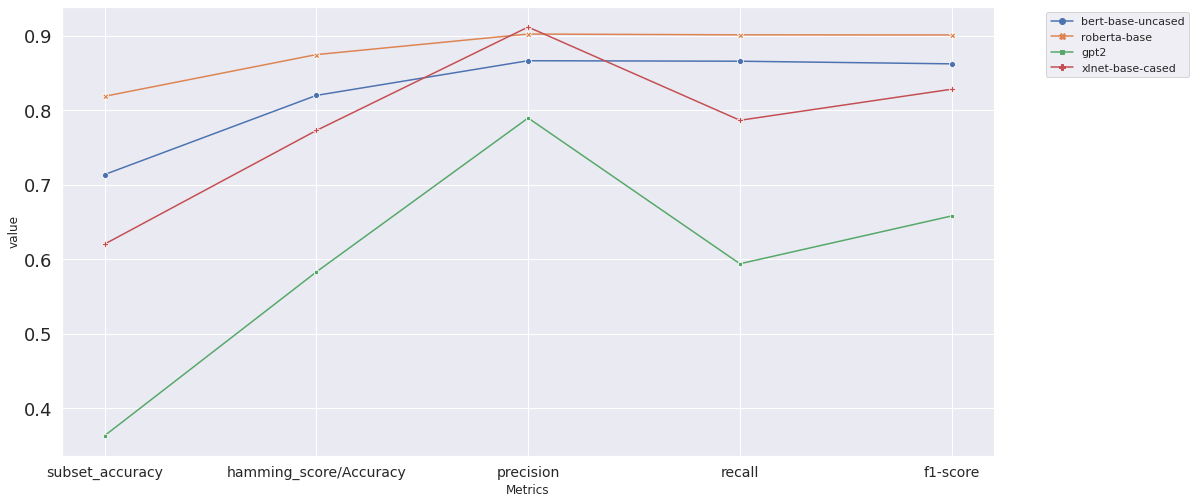
\includegraphics[width=1\textwidth]{thesis/figures/summary.png}
    \caption{Sample average results of language models }
    \label{fig:model_wise_group_LM}
\end{figure}
% A subset of sample-based metrics with similar scales have been compiled and can be seen in the figure \ref{fig:model_wise_group_LM}.
\subsubsection{Roberta}
Overall, Roberta is the best performing language model. Considering subset accuracy, roberta could achieve an accuracy of 81\%, which is 12.8\% more than the bert (next best to Roberta) and 40.2\% greater than the best performing baseline model (decision tree with tf\_idf). From the figure \ref{fig:model_wise_group_LM} it is clear that except for the sample average precision of xlnet, which is 1.04\% greater than Roberta, it is the best performing model among others. Coming to label-based measure \ref{LMreports} micro and macro average, it follows the same pattern that in the sample average results, where the precision of xlnet is slightly better but the recall and f1-score of roberta is highest for both the measures. The macro average f1-score (90.75\%) is 0.69\% higher than sample average score. The micro average f1-score (89.17\%) is 1.04\% less than sample average f1-score. Micro and macro average scores are based on the label wise scores of language models shown in the table \ref{tab:Per-Label-precision-recall-f-measure}. The  f1-score of 'stereotype' class is 83.3\%, which is 8.85\% greater than bert 'stereotype' class f1-score and 13.17\% greater than xlnet 'stereotype' class f1-score. The f1-scores of stereotype and anti-stereotype on an average are 10 to 20\% lower when compared to scores of bias types (ethnicity, gender, profession, religion), which indicates that the classifier is better at identifying bias types. The f1-score of 'unrelated' class (97.7\%) is significantly higher than f1-scores of stereotype and anti-stereotype. One of the characteristic properties of roberta are its hyperparameters used for training. The hyperparameter search results of roberta \ref{tab:search_results} were different with higher number of epochs and a different learning rate, which might be one of the reasons for having high scores. Another significant property of roberta is its training data. Apart from the training data used for bert, it was trained on CC-News (English portion of Common crawl newsdataset, 76 GB), openWebText (web content extracted from URLs shared on Reddit with atleast three upvotes. 38 GB). Since, it's trained on Reddit which has several subreddits related to target terms in stereoset \cite{nadeem2020stereoset}, this might have some effect on the classification as the knowledge is being transferred. 

% \begin{itemize}
%     \item Roberta: The advantages of using transfer learning and language models is the robustness of the model apart from the effectiveness.
% \end{itemize}

\subsubsection{Bert}
Bert is the next best performing language model. As can be seen from the figure \ref{fig:model_wise_group_LM}, there is a marginal difference in the performance betweeen roberta and bert. The subset accuracy of bert is 71.37\% which is 13.08\% higher than xlnet and 12.8\% less than roberta. When compared to best performing baseline model (decision tree with tf\_idf), bert subset accuracy is 18.21\% higher. The sample average scores of roberta and bert vary by around 4.49\% for precision, recall, f1-score. Coming to label based metrics such as micro and macro average precision, recall and f-measure \ref{LMreports}; the micro  average f1-score (87.39\%)  is 1.33\% greater than sample average f1-score while macro average f1-score (84.95\%) is 1.49\% less when compared to sample average f1-score. Micro and macro average scores are based on the label wise scores of language models shown in the table \ref{tab:Per-Label-precision-recall-f-measure}. As can be observed, the scores of bias categories are on an average 33.4\% higher than scores of stereotype and anti-stereotype. The f1-score of 'unrelated' class (98.1\%) is significantly higher than f1-scores of stereotype and anti-stereotype. The f1-score of 'stereotype' class is 75.97\% while anti-stereotype is 63.45\% which is around 8 to 9\% less than roberta. The variation of scores between roberta and bert may be due to the fact that roberta was trained for 5 epochs while other models including bert was trained for 2 epochs. Since, roberta is an optimized version of bert, similar behavior is observed. 

\subsubsection{Xlnet}
Xlnet language model has a subset accuracy of 62\% which is 13.08\% less than bert and 24.2\% less than roberta. As can be seen from the figure \ref{fig:model_wise_group_LM}, the precision of xlnet is higher than roberta by around 1.04\%, but the recall is significantly lower than roberta and bert. The reason for such high precision could be based on the language model architecture. As xlnet is a generalized autoregressive model which incorporates bidirectional context on the pure autoregressive model, an effect can be observed in the precision being very close to that of auto encoding models (bert and roberta) which also incorporate bidirectionality.  Coming to the label based metrics, micro, macro average scores \ref{LMreports}, the scores show same trend as in sample average with no significant changes. Coming to the label wise results shown in table \ref{tab:Per-Label-precision-recall-f-measure}, the f1-score of 'stereotype' class is around 72.36 \%  which is 4.74\% less than bert; while 'anti-stereotype' class has 53.56\% which is 15.59\% less than bert. On average the stereotype and anti-stereotype scores are 30\% less when compared to bias categories. The f1-score of 'unrelated' class (96.4\%) is significantly higher than f1-scores of stereotype and anti-stereotype.

\subsubsection{GPT-2}
GPT-2 is the worst performing model among language models. As can be seen from the figure \ref{fig:model_wise_group_LM} it has the lowest subset accuracy of 36.31\% when compared to other language models, and it's significantly lower than the best performing baseline (decision tree using \acrshort{tfidf}) by 60.75\%. The significant low performance might be due to language model architecture. GPT-2 is purely left to right autoregressive model trained for language modeling task and hence using it for text classification might be the reason for having such low performance. The sample average precision is 78.97\% which is 9.7\% lower than bert precision, but recall is significantly lower (45.78\% than bert) and  (32.4\% than xlnet) which leads to a f1-score of 65.82\% (13.19\% lower than decision tree using \acrshort{tfidf}). Coming to label based metrics \ref{LMreports}, micro and macro average f1-score remain almost the same. The f1-score of 'stereotype' is 47.45 \% while of 'anti-stereotype' is 20.7\% which are the lowest scores among others. 

\subsubsection{Summary}
On an average, language model performs significantly better than feature base models with roberta having a subset accuracy which is 40.2\% greater than the decision tree baseline. Next to roberta is bert and followed by xlnet. GPT-2 is the worst performing model. The f1-scores of stereotype, anti-stereotype of language models seems to be around 10 to 20 \% lower when compared to bias categories. The f1-score of 'Unrelated' is significantly better for all the models.

\begin{landscape}
\begin{table}[]
\resizebox{\columnwidth}{!}{%
\begin{tabular}{@{}lllllllll@{}}
\toprule
Model\_name &
  Metrics &
  Ethnicity &
  Gender &
  Profession &
  Religion &
  Anti-stereotype &
  Stereotype &
  Unrelated \\ \midrule
\multicolumn{1}{|l|}{\multirow{4}{*}{bert\_base\_uncased}} &
  \multicolumn{1}{l|}{precision} &
  \multicolumn{1}{l|}{0.9773299748110831} &
  \multicolumn{1}{l|}{0.8960573476702509} &
  \multicolumn{1}{l|}{0.9004149377593361} &
  \multicolumn{1}{l|}{0.9897610921501706} &
  \multicolumn{1}{l|}{0.6714490674318508} &
  \multicolumn{1}{l|}{0.7202680067001676} &
  \multicolumn{1}{l|}{0.9935064935064936} \\ \cmidrule(l){2-9} 
\multicolumn{1}{|l|}{} &
  \multicolumn{1}{l|}{recall} &
  \multicolumn{1}{l|}{0.9897959183673469} &
  \multicolumn{1}{l|}{0.8223684210526315} &
  \multicolumn{1}{l|}{0.9293361884368309} &
  \multicolumn{1}{l|}{0.9897610921501706} &
  \multicolumn{1}{l|}{0.6015424164524421} &
  \multicolumn{1}{l|}{0.8037383177570093} &
  \multicolumn{1}{l|}{0.9622641509433962} \\ \cmidrule(l){2-9} 
\multicolumn{1}{|l|}{} &
  \multicolumn{1}{l|}{f1-score} &
  \multicolumn{1}{l|}{0.9835234474017743} &
  \multicolumn{1}{l|}{0.8576329331046311} &
  \multicolumn{1}{l|}{0.9146469968387777} &
  \multicolumn{1}{l|}{0.9897610921501706} &
  \multicolumn{1}{l|}{0.6345762711864408} &
  \multicolumn{1}{l|}{0.7597173144876326} &
  \multicolumn{1}{l|}{0.9776357827476039} \\ \cmidrule(l){2-9} 
\multicolumn{1}{|l|}{} &
  \multicolumn{1}{l|}{support} &
  \multicolumn{1}{l|}{784.0} &
  \multicolumn{1}{l|}{304.0} &
  \multicolumn{1}{l|}{467.0} &
  \multicolumn{1}{l|}{293.0} &
  \multicolumn{1}{l|}{778.0} &
  \multicolumn{1}{l|}{1070.0} &
  \multicolumn{1}{l|}{636.0} \\ \midrule
\multicolumn{1}{|l|}{\multirow{4}{*}{roberta-base}} &
  \multicolumn{1}{l|}{precision} &
  \multicolumn{1}{l|}{0.9834394904458599} &
  \multicolumn{1}{l|}{0.8778135048231511} &
  \multicolumn{1}{l|}{0.9261603375527426} &
  \multicolumn{1}{l|}{0.9931740614334471} &
  \multicolumn{1}{l|}{0.7858176555716353} &
  \multicolumn{1}{l|}{0.8038194444444444} &
  \multicolumn{1}{l|}{0.9935587761674718} \\ \cmidrule(l){2-9} 
\multicolumn{1}{|l|}{} &
  \multicolumn{1}{l|}{recall} &
  \multicolumn{1}{l|}{0.9846938775510204} &
  \multicolumn{1}{l|}{0.8980263157894737} &
  \multicolumn{1}{l|}{0.9400428265524625} &
  \multicolumn{1}{l|}{0.9931740614334471} &
  \multicolumn{1}{l|}{0.6979434447300771} &
  \multicolumn{1}{l|}{0.8654205607476636} &
  \multicolumn{1}{l|}{0.970125786163522} \\ \cmidrule(l){2-9} 
\multicolumn{1}{|l|}{} &
  \multicolumn{1}{l|}{f1-score} &
  \multicolumn{1}{l|}{0.9840662842574888} &
  \multicolumn{1}{l|}{0.8878048780487804} &
  \multicolumn{1}{l|}{0.9330499468650373} &
  \multicolumn{1}{l|}{0.9931740614334471} &
  \multicolumn{1}{l|}{0.7392784206943499} &
  \multicolumn{1}{l|}{0.8334833483348336} &
  \multicolumn{1}{l|}{0.9817024661893397} \\ \cmidrule(l){2-9} 
\multicolumn{1}{|l|}{} &
  \multicolumn{1}{l|}{support} &
  \multicolumn{1}{l|}{784.0} &
  \multicolumn{1}{l|}{304.0} &
  \multicolumn{1}{l|}{467.0} &
  \multicolumn{1}{l|}{293.0} &
  \multicolumn{1}{l|}{778.0} &
  \multicolumn{1}{l|}{1070.0} &
  \multicolumn{1}{l|}{636.0} \\ \midrule
\multicolumn{1}{|l|}{\multirow{4}{*}{xlnet-base-cased}} &
  \multicolumn{1}{l|}{precision} &
  \multicolumn{1}{l|}{0.96625} &
  \multicolumn{1}{l|}{0.8951310861423221} &
  \multicolumn{1}{l|}{0.9014989293361885} &
  \multicolumn{1}{l|}{0.993103448275862} &
  \multicolumn{1}{l|}{0.8062015503875969} &
  \multicolumn{1}{l|}{0.8386699507389163} &
  \multicolumn{1}{l|}{0.9916943521594684} \\ \cmidrule(l){2-9} 
\multicolumn{1}{|l|}{} &
  \multicolumn{1}{l|}{recall} &
  \multicolumn{1}{l|}{0.985969387755102} &
  \multicolumn{1}{l|}{0.7861842105263158} &
  \multicolumn{1}{l|}{0.9014989293361885} &
  \multicolumn{1}{l|}{0.9829351535836177} &
  \multicolumn{1}{l|}{0.40102827763496146} &
  \multicolumn{1}{l|}{0.6364485981308411} &
  \multicolumn{1}{l|}{0.9386792452830188} \\ \cmidrule(l){2-9} 
\multicolumn{1}{|l|}{} &
  \multicolumn{1}{l|}{f1-score} &
  \multicolumn{1}{l|}{0.9760101010101009} &
  \multicolumn{1}{l|}{0.8371278458844135} &
  \multicolumn{1}{l|}{0.9014989293361885} &
  \multicolumn{1}{l|}{0.9879931389365352} &
  \multicolumn{1}{l|}{0.5356223175965665} &
  \multicolumn{1}{l|}{0.7236981934112645} &
  \multicolumn{1}{l|}{0.9644588045234248} \\ \cmidrule(l){2-9} 
\multicolumn{1}{|l|}{} &
  \multicolumn{1}{l|}{support} &
  \multicolumn{1}{l|}{784.0} &
  \multicolumn{1}{l|}{304.0} &
  \multicolumn{1}{l|}{467.0} &
  \multicolumn{1}{l|}{293.0} &
  \multicolumn{1}{l|}{778.0} &
  \multicolumn{1}{l|}{1070.0} &
  \multicolumn{1}{l|}{636.0} \\ \midrule
\multicolumn{1}{|l|}{\multirow{4}{*}{gpt2}} &
  \multicolumn{1}{l|}{precision} &
  \multicolumn{1}{l|}{0.9219178082191781} &
  \multicolumn{1}{l|}{0.8918918918918919} &
  \multicolumn{1}{l|}{0.8039647577092511} &
  \multicolumn{1}{l|}{0.9745454545454545} &
  \multicolumn{1}{l|}{0.5833333333333334} &
  \multicolumn{1}{l|}{0.8333333333333334} &
  \multicolumn{1}{l|}{0.9515260323159784} \\ \cmidrule(l){2-9} 
\multicolumn{1}{|l|}{} &
  \multicolumn{1}{l|}{recall} &
  \multicolumn{1}{l|}{0.8584183673469388} &
  \multicolumn{1}{l|}{0.4342105263157895} &
  \multicolumn{1}{l|}{0.7815845824411135} &
  \multicolumn{1}{l|}{0.9146757679180887} &
  \multicolumn{1}{l|}{0.12596401028277635} &
  \multicolumn{1}{l|}{0.3317757009345794} &
  \multicolumn{1}{l|}{0.8333333333333334} \\ \cmidrule(l){2-9} 
\multicolumn{1}{|l|}{} &
  \multicolumn{1}{l|}{f1-score} &
  \multicolumn{1}{l|}{0.8890356671070013} &
  \multicolumn{1}{l|}{0.5840707964601769} &
  \multicolumn{1}{l|}{0.7926167209554832} &
  \multicolumn{1}{l|}{0.9436619718309859} &
  \multicolumn{1}{l|}{0.20718816067653276} &
  \multicolumn{1}{l|}{0.4745989304812835} &
  \multicolumn{1}{l|}{0.8885163453478626} \\ \cmidrule(l){2-9} 
\multicolumn{1}{|l|}{} &
  \multicolumn{1}{l|}{support} &
  \multicolumn{1}{l|}{784.0} &
  \multicolumn{1}{l|}{304.0} &
  \multicolumn{1}{l|}{467.0} &
  \multicolumn{1}{l|}{293.0} &
  \multicolumn{1}{l|}{778.0} &
  \multicolumn{1}{l|}{1070.0} &
  \multicolumn{1}{l|}{636.0} \\ \bottomrule
\end{tabular}%
}
\caption{Label wise precision, recall, f1score and support measures}
\label{tab:Per-Label-precision-recall-f-measure}
\end{table}
\end{landscape}

\subsection{Evaluation of Baselines}
% \begin{figure}[h!]
%     \centering
%     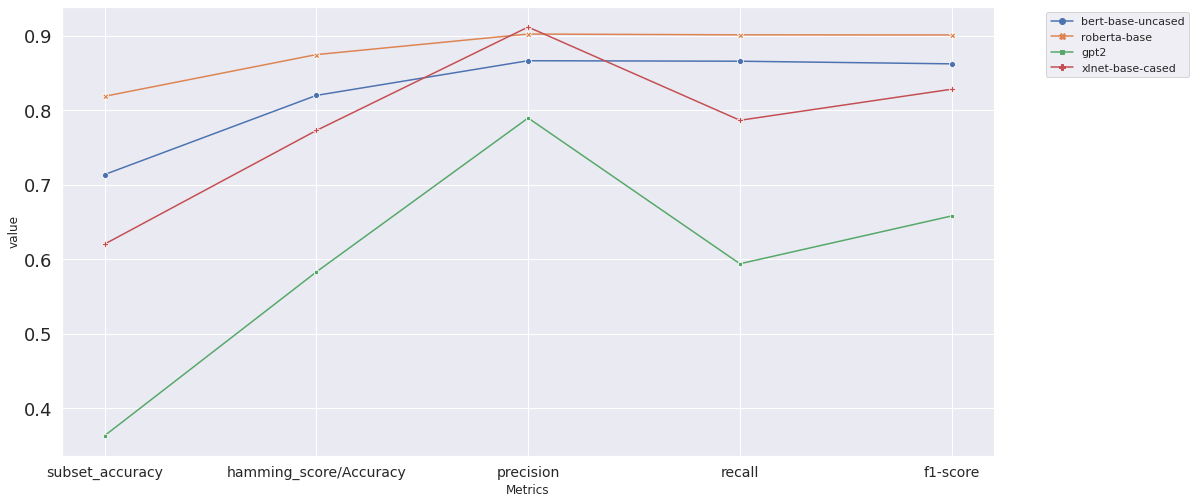
\includegraphics[width=1\textwidth]{thesis/figures/summary.png}
%     \caption{Sample average metrics summary results of language models }
%     \label{fig:model_wise_group_LM}
% \end{figure}
\begin{figure}[h!]
    \centering
    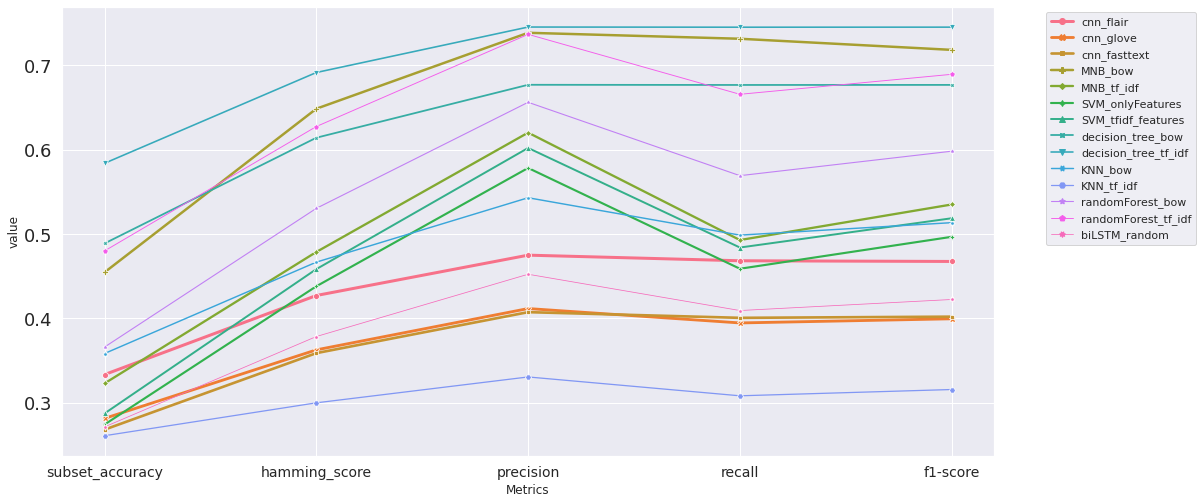
\includegraphics[width=1\textwidth]{thesis/figures/Baslines.png}
    \caption{Sample average metrics summary results of baseline models }
    \label{fig:model_wise_group_baseline}
\end{figure}
% \begin{itemize}
%     \item MNB and decision tree: Through training these models is far cost-effective, the robustness of the model remains an issue. 
%     \item The results on the test set states that these machine learning models are performing well on explicit features, but when tested with random samples, it might fail miserably. 
% \end{itemize}
Figure \ref{fig:model_wise_group_baseline} shows a cumulative view of different baselines tested. Out of the many models which were experimented with different features, decision tree using \acrshort{tfidf} is the best performing model, followed by multinomial naive Bayes with bag of words features and random forest with tf\_idf features. These models have achieved a significant performance (46.04\% higher) when compared to deep learning models. A pattern that could be observed is that tree based models have outperformed other models. Another interesting point is that bag of words and tf\_idf features could outperform pre-trained word embedding models, including flair, which is a contextual word embedding model. Decision tree classifier algorithm works by forming a hierarchical structure of data using some rules/questions set on the features associated to the data\cite{kingsford2008decision}. The higher performance of tree based models could be due to the hierarchical structure of the features and their correlations, as shown in the figure \ref{fig:decision_tree_baseline}. This shows that the stereotypical data is hierarchical in structure. One more interesting point is that decision tree, random forests and k-neighbors algorithms inherently support multi label classification\footnote{\url{https://scikit-learn.org/stable/modules/multiclass.html}}. The other baseline models are transformed using binary relevance technique, which decomposes the multi label to multiple binary classification problems. Comparing the worst performing language model (GPT-2) to the best performing baseline model (decision tree with tf\_idf features); decision tree has 60.75\% higher subset accuracy than gpt-2.  Coming to sample average f1-score, decision tree has 13.19\% higher f1-score than gpt-2, where the recall of gpt-2 was much lower by 25.41\% when compared to decision tree. Coming to label based metrics \ref{LMreports}, an interesting observation is that, multinomial naive bayes with tf\_idf features has the best micro-average f1-score (72.63\%), while, decision tree with tf\_idf features has the best macro-average f1-score (74.9\%) followed by multinomial naive bayes with tf\_idf with a difference of 0.4\%. Difference in results of different averaging technique might be due to the influence of class imbalance in the dataset, which might influences the decision of the underlying algorithm as well. 
\pagebreak
 
% Please add the following required packages to your document preamble:
% \usepackage{booktabs}
% \usepackage{multirow}
% \usepackage{graphicx}
% \pagebreak
% Please add the following required packages to your document preamble:
% \usepackage{booktabs}
% \usepackage{multirow}
% \usepackage{graphicx}
% Please add the following required packages to your document preamble:
% \usepackage{booktabs}
% \usepackage{multirow}
% \usepackage{graphicx}
\begin{table}[]
\resizebox{\textwidth}{!}{%
\begin{tabular}{@{}clllllllll@{}}
\toprule
Model\_name &
  Text feature &
  Metrics &
  Ethnicity &
  gender &
  profession &
  religion &
  Anti-stereotype &
  stereotype &
  unrelated \\ \midrule
\multicolumn{1}{|c|}{\multirow{4}{*}{Decision\_tree}} &
  \multicolumn{1}{l|}{\multirow{4}{*}{Tf\_idf}} &
  \multicolumn{1}{l|}{precision} &
  \multicolumn{1}{l|}{0.8659003831417624} &
  \multicolumn{1}{l|}{0.7247386759581882} &
  \multicolumn{1}{l|}{0.823404255319149} &
  \multicolumn{1}{l|}{0.9163498098859315} &
  \multicolumn{1}{l|}{0.47724477244772445} &
  \multicolumn{1}{l|}{0.6224696356275303} &
  \multicolumn{1}{l|}{0.869309838472834} \\ \cmidrule(l){3-10} 
\multicolumn{1}{|c|}{} &
  \multicolumn{1}{l|}{} &
  \multicolumn{1}{l|}{recall} &
  \multicolumn{1}{l|}{0.8647959183673469} &
  \multicolumn{1}{l|}{0.6864686468646864} &
  \multicolumn{1}{l|}{0.828693790149893} &
  \multicolumn{1}{l|}{0.8225255972696246} &
  \multicolumn{1}{l|}{0.49935649935649934} &
  \multicolumn{1}{l|}{0.5747663551401869} &
  \multicolumn{1}{l|}{0.9293563579277865} \\ \cmidrule(l){3-10} 
\multicolumn{1}{|c|}{} &
  \multicolumn{1}{l|}{} &
  \multicolumn{1}{l|}{f1-score} &
  \multicolumn{1}{l|}{0.8653477983407786} &
  \multicolumn{1}{l|}{0.7050847457627119} &
  \multicolumn{1}{l|}{0.8260405549626468} &
  \multicolumn{1}{l|}{0.8669064748201438} &
  \multicolumn{1}{l|}{0.48805031446540875} &
  \multicolumn{1}{l|}{0.597667638483965} &
  \multicolumn{1}{l|}{0.8983308042488619} \\ \cmidrule(l){3-10} 
\multicolumn{1}{|c|}{} &
  \multicolumn{1}{l|}{} &
  \multicolumn{1}{l|}{support} &
  \multicolumn{1}{l|}{784.0} &
  \multicolumn{1}{l|}{303.0} &
  \multicolumn{1}{l|}{467.0} &
  \multicolumn{1}{l|}{293.0} &
  \multicolumn{1}{l|}{777.0} &
  \multicolumn{1}{l|}{1070.0} &
  \multicolumn{1}{l|}{637.0} \\ \bottomrule
\end{tabular}%
}
\caption{Label wise scores of decision trees}
\label{tab:Label_wise_decision tree}
\end{table}

\begin{table}[h!]
\resizebox{\textwidth}{!}{%
\begin{tabular}{@{}ccllllllll@{}}
\toprule
\multicolumn{1}{l}{Model name} &
  \multicolumn{1}{l}{Text feature} &
  Metrics &
  Ethnicity &
  gender &
  profession &
  religion &
  Anti-stereotype &
  stereotype &
  unrelated \\ \midrule
\multicolumn{1}{|c|}{\multirow{4}{*}{RandomForest}} &
  \multicolumn{1}{c|}{\multirow{4}{*}{Tf\_idf}} &
  \multicolumn{1}{l|}{precision} &
  \multicolumn{1}{l|}{0.9486823855755895} &
  \multicolumn{1}{l|}{0.9512195121951219} &
  \multicolumn{1}{l|}{0.8896882494004796} &
  \multicolumn{1}{l|}{0.9908256880733946} &
  \multicolumn{1}{l|}{0.4063157894736842} &
  \multicolumn{1}{l|}{0.5949074074074074} &
  \multicolumn{1}{l|}{0.911353032659409} \\ \cmidrule(l){3-10} 
\multicolumn{1}{|c|}{} &
  \multicolumn{1}{c|}{} &
  \multicolumn{1}{l|}{recall} &
  \multicolumn{1}{l|}{0.8724489795918368} &
  \multicolumn{1}{l|}{0.5148514851485149} &
  \multicolumn{1}{l|}{0.7944325481798715} &
  \multicolumn{1}{l|}{0.7372013651877133} &
  \multicolumn{1}{l|}{0.2483912483912484} &
  \multicolumn{1}{l|}{0.4803738317757009} &
  \multicolumn{1}{l|}{0.9199372056514914} \\ \cmidrule(l){3-10} 
\multicolumn{1}{|c|}{} &
  \multicolumn{1}{c|}{} &
  \multicolumn{1}{l|}{f1-score} &
  \multicolumn{1}{l|}{0.908970099667774} &
  \multicolumn{1}{l|}{0.6680942184154176} &
  \multicolumn{1}{l|}{0.8393665158371041} &
  \multicolumn{1}{l|}{0.8454011741682973} &
  \multicolumn{1}{l|}{0.3083067092651757} &
  \multicolumn{1}{l|}{0.531540847983454} &
  \multicolumn{1}{l|}{0.9156249999999999} \\ \cmidrule(l){3-10} 
\multicolumn{1}{|c|}{} &
  \multicolumn{1}{c|}{} &
  \multicolumn{1}{l|}{support} &
  \multicolumn{1}{l|}{784.0} &
  \multicolumn{1}{l|}{303.0} &
  \multicolumn{1}{l|}{467.0} &
  \multicolumn{1}{l|}{293.0} &
  \multicolumn{1}{l|}{777.0} &
  \multicolumn{1}{l|}{1070.0} &
  \multicolumn{1}{l|}{637.0} \\ \bottomrule
\end{tabular}%
}
\caption{Label-wise scores of Random forest}
\label{tab:Label-wise-random-forest}
\end{table}

\begin{table}[h!]
\resizebox{\textwidth}{!}{%
\begin{tabular}{@{}ccllllllll@{}}
\toprule
\multicolumn{1}{l}{Model name} &
  \multicolumn{1}{l}{Text feature} &
  Metrics &
  Ethnicity &
  gender &
  profession &
  religion &
  Anti-stereotype &
  stereotype &
  unrelated \\ \midrule
\multicolumn{1}{|c|}{\multirow{4}{*}{MNB}} &
  \multicolumn{1}{c|}{\multirow{4}{*}{Bow}} &
  \multicolumn{1}{l|}{precision} &
  \multicolumn{1}{l|}{0.8687116564417178} &
  \multicolumn{1}{l|}{0.6818181818181818} &
  \multicolumn{1}{l|}{0.780439121756487} &
  \multicolumn{1}{l|}{0.8597122302158273} &
  \multicolumn{1}{l|}{0.49623250807319697} &
  \multicolumn{1}{l|}{0.6677524429967426} &
  \multicolumn{1}{l|}{0.9606003752345216} \\ \cmidrule(l){3-10} 
\multicolumn{1}{|c|}{} &
  \multicolumn{1}{c|}{} &
  \multicolumn{1}{l|}{recall} &
  \multicolumn{1}{l|}{0.9030612244897959} &
  \multicolumn{1}{l|}{0.6435643564356436} &
  \multicolumn{1}{l|}{0.8372591006423983} &
  \multicolumn{1}{l|}{0.8156996587030717} &
  \multicolumn{1}{l|}{0.5933075933075933} &
  \multicolumn{1}{l|}{0.5747663551401869} &
  \multicolumn{1}{l|}{0.8037676609105181} \\ \cmidrule(l){3-10} 
\multicolumn{1}{|c|}{} &
  \multicolumn{1}{c|}{} &
  \multicolumn{1}{l|}{f1-score} &
  \multicolumn{1}{l|}{0.8855534709193245} &
  \multicolumn{1}{l|}{0.6621392190152802} &
  \multicolumn{1}{l|}{0.8078512396694214} &
  \multicolumn{1}{l|}{0.8371278458844134} &
  \multicolumn{1}{l|}{0.540445486518171} &
  \multicolumn{1}{l|}{0.6177800100452036} &
  \multicolumn{1}{l|}{0.8752136752136753} \\ \cmidrule(l){3-10} 
\multicolumn{1}{|c|}{} &
  \multicolumn{1}{c|}{} &
  \multicolumn{1}{l|}{support} &
  \multicolumn{1}{l|}{784.0} &
  \multicolumn{1}{l|}{303.0} &
  \multicolumn{1}{l|}{467.0} &
  \multicolumn{1}{l|}{293.0} &
  \multicolumn{1}{l|}{777.0} &
  \multicolumn{1}{l|}{1070.0} &
  \multicolumn{1}{l|}{637.0} \\ \bottomrule
\end{tabular}%
}
\caption{Label-wise scores of Multinomial Naive Bayes}
\label{tab:Label-wise-Naiye-Bayes}
\end{table}

Coming to the label wise results of top performing models, As seen in the table \ref{tab:Label_wise_decision tree}, the multinomial naive bayes has higher stereotype and anti-stereotype f1-scores marginally (3.24\%) better than decision trees when considering anti-stereotype and stereotype but for other 4 categories (bias types), decision tree scores are a bit higher, this is the reason for decision trees having higher macro average f1-score and multinomial naive bayes having higher micro average f1-score. One characteristic property of random forests is that it has lowest scores for 'anti-stereotype' class. Comparing text features i.e. bag of words and term frequency- inverse document frequency features and pre-trained word embedding models, pre-trained embeddings with deep learning model could not achieve the significant results. The characteristics of stereotypical data used might have an impact, which made models such as multinomial naive bayes with bag of words features achieve significant results. overall, the influence of underlying algorithm and the data characteristics has an impact on the results. Considering multinomial naive bayes model, the recall value of anti-stereotype with tf\_idf feature had a drop of 72.88\% when compared to multinomial naive bayes with bag of words feature. This might be due to the fact that multinomial naive bayes assumes documents as bag of words and uses word frequency counts into account.

\subsubsection{Summary}
Overall, the feature based baseline models could achieve good performance in regard to cost of training. Decision tress with term frequency-inverse document frequency (Tf\_idf) model has the highest subset accuracy and overall is the best performing model. This is followed by multinomial naive bayes with bag of words feature and random forests with Tf\_idf feature. Decision tree model outperformed gpt-2 language model with respect to the subset accuracy. The worst performing model is k nearest neighbor algorithm with bag of words feature. Deep learning models with pre-trained word embeddings have a marginal impact and could not outperform the simple tree based models. 

\pagebreak

\section{Qualitative analysis} \label{Qualitative_analysis}
In addition to the quantitative analysis, this section covers the qualitative aspects and insights gained when testing on some manually generated samples. The best performing model from both the approaches are taken and compared on different aspects. Roberta model is selected from fine-tuning based approach and decision tree with tf\_idf features is selected from feature based approach.

\subsection{Fine-tuning based approach}

\subsubsection{Efficiency}
\subsubsection{Error analysis}
\subsubsection{Manual evaluation}
\begin{itemize}
    \item test associations (stereo, anti-stereo, unrelated)
    \item Test explicit (test association), implicit stereotypes (test target)
\end{itemize}
\subsection{Feature-based approach}

\subsubsection{Efficiency}
\subsubsection{Error analysis}
\subsubsection{Manual evaluation}
\begin{itemize}
    \item test associations (stereo, anti-stereo, unrelated)
    \item Test explicit (test association), implicit stereotypes (test target)
\end{itemize}
% \begin{itemize}
%     \item Interpretation of results and Selecting best performing model 
%     \item Best performing model discussion with manual sentences (Test cases ) 
%     \begin{itemize}
%         \item Effectiveness (Metrics)
%         \item Efficiency (time)
%         \item Test Explicit(Associations to stereo attribute) and implicit (Analogies) stereotypes
%         \begin{itemize}
%             \item Explicit stereotypes : Overt expression of target with attribute, e.g. target : African, stereotypic attribute : good at running
%             \item Implicit stereotypes : Subtle expression of stereotypes where the target is an instance of target and where the attribute may be synonymous as well
%             e.g. Target : African name, stereotypic attribute :  good at running 
%         \end{itemize} 
%         \item Test for explicit stereotypical bias statements  (stereotypical, anti-stereotypical and unrelated)
%         \item Test by changing target other than the provided in dataset 
%         \item Manual evaluation with respect to selected arguments (IBM dataset) and analysis with respect to user study 
%     \end{itemize}
% \end{itemize}

\begin{landscape}
\begin{figure}[h!]
    \centering
    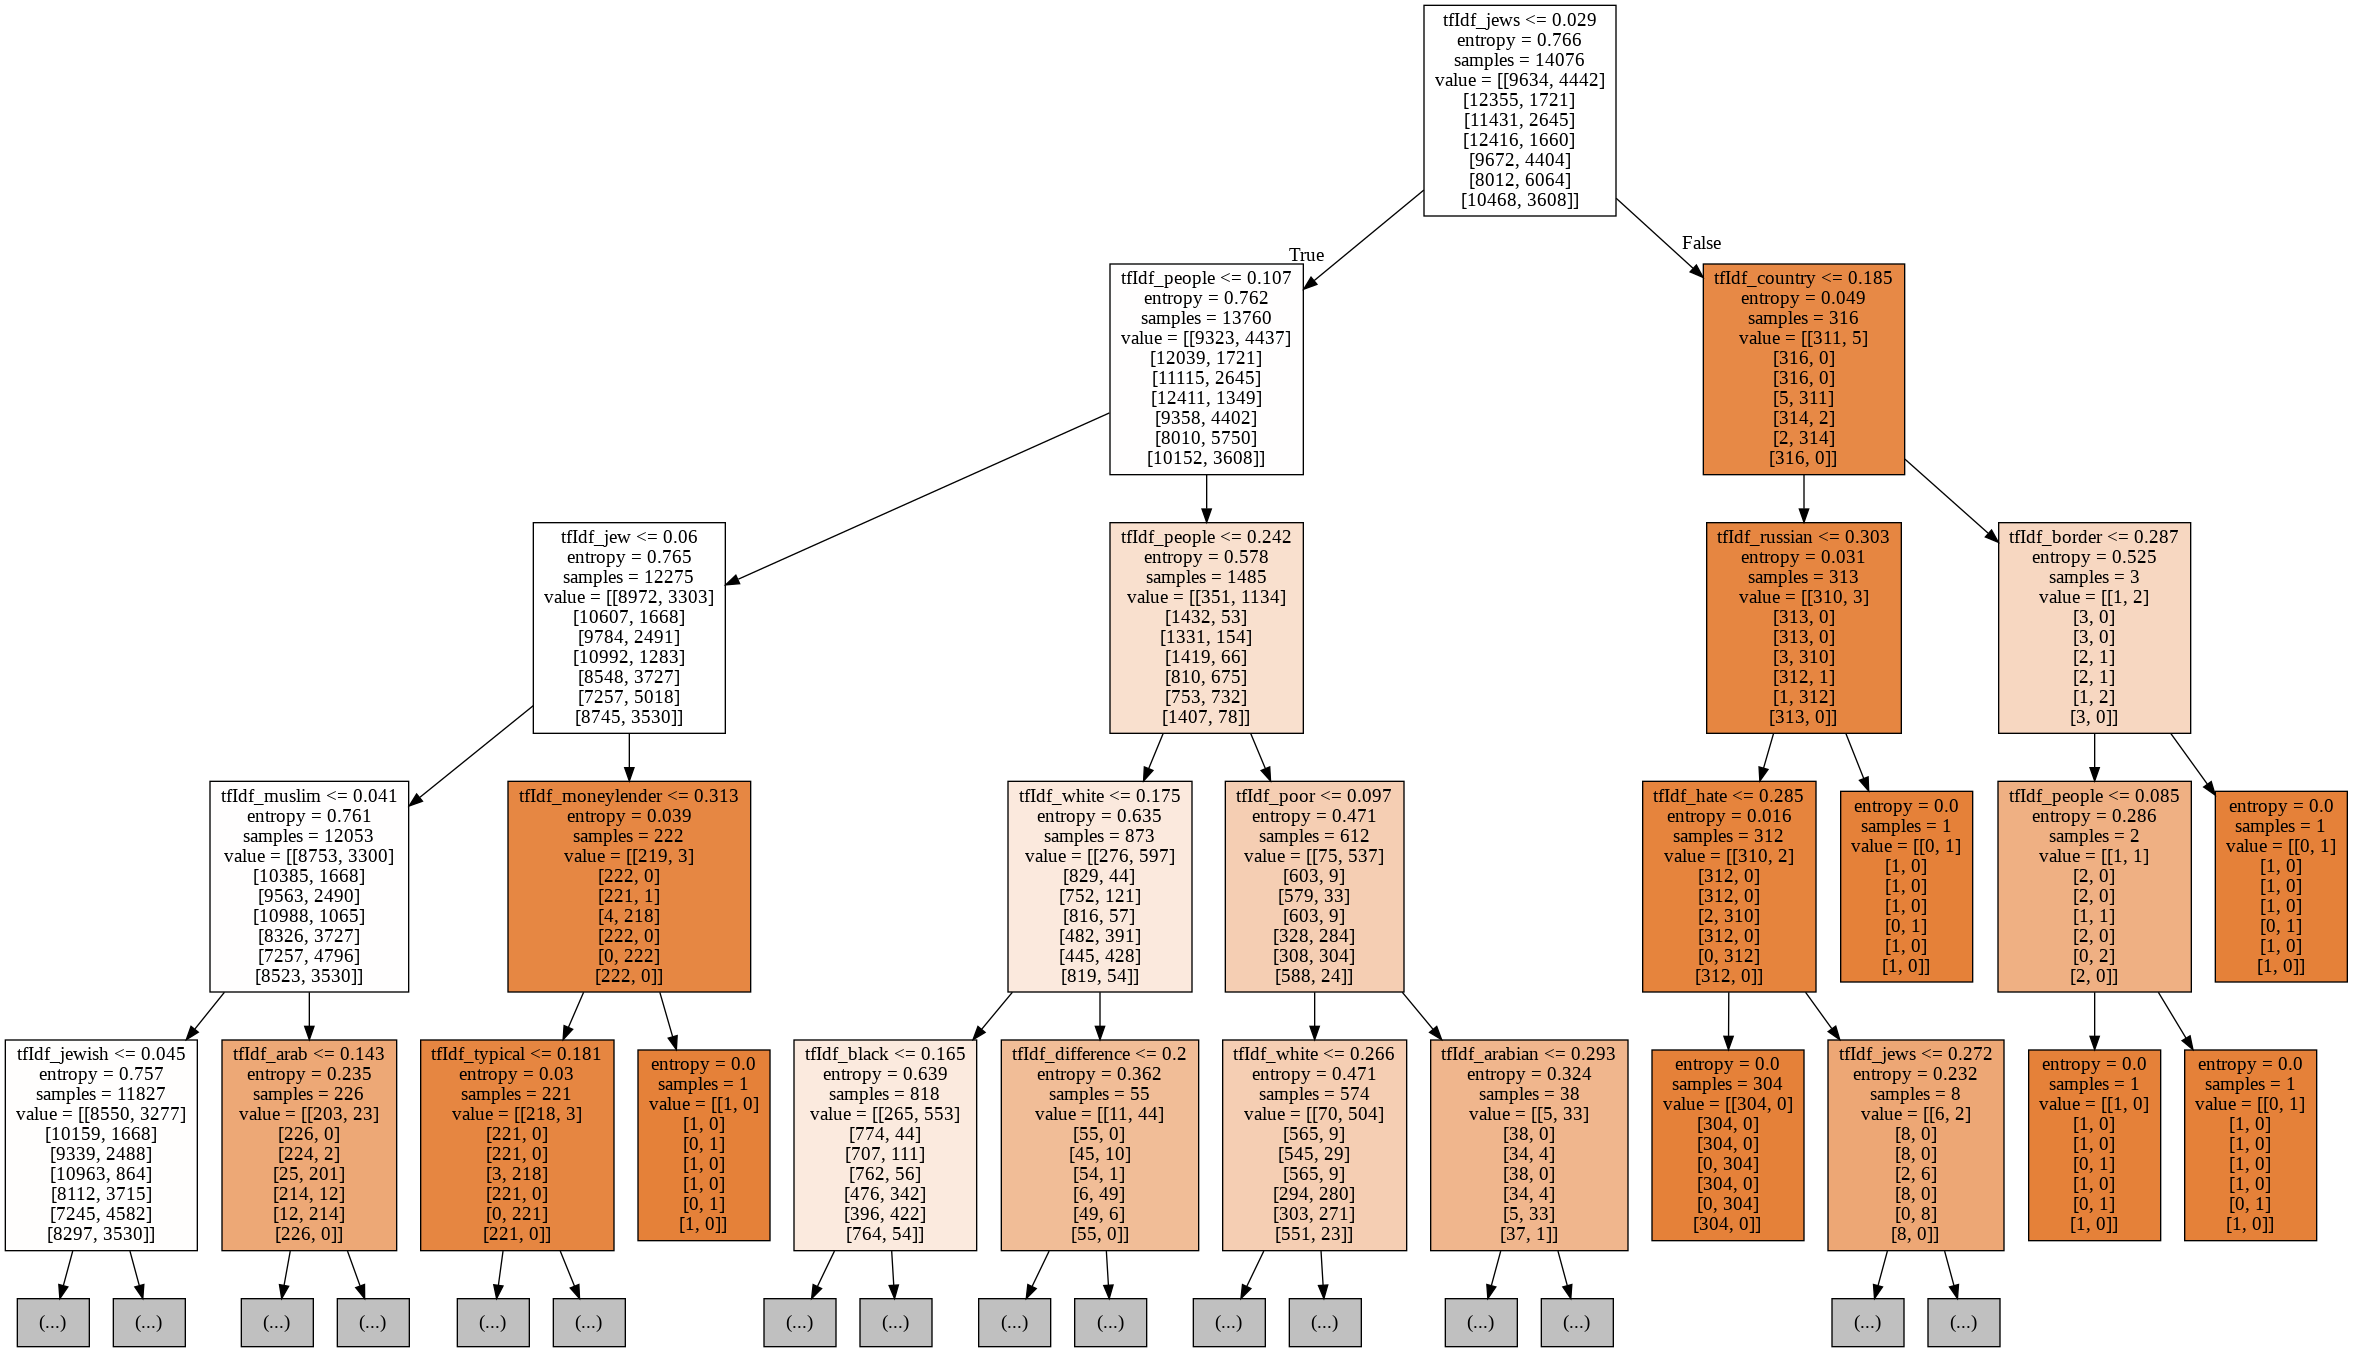
\includegraphics[width=1\textwidth]{thesis/figures/decision_tree_graphivz.png}
    \caption{The hierarchical structure of decision tree with tf\_idf features}
    \label{fig:decision_tree_baseline}
\end{figure}
\end{landscape}